\documentclass[11pt]{article}
\usepackage[margin=1in]{geometry}
\usepackage{amsmath,amssymb,bm}
\usepackage{booktabs}
\usepackage{enumitem}
\usepackage{graphicx}
\usepackage{hyperref}
\pdfstringdefDisableCommands{%
  \def\vect#1{#1}%
  \def\ddot#1{#1_ddot}%
  \def\dot#1{#1_dot}%
}
\usepackage{tikz}
\usetikzlibrary{arrows.meta,decorations.pathmorphing,patterns,calc}

\newcommand{\dd}{\mathrm{d}}
\newcommand{\vect}[1]{\bm{#1}}

\title{Derivation of a 7-DOF Full Car Suspension Model}
\author{J.C.\ Vaught}
\date{January 2026}

\begin{document}
\maketitle
\tableofcontents
\newpage

%======================================================================
\section{Model Description and Coordinate System}
%======================================================================

The 7-DOF full car model captures the essential dynamics of a passenger vehicle's vertical/angular response to road inputs. The model treats the car body (sprung mass) as a rigid body with three degrees of freedom and each wheel assembly (unsprung mass) as a point mass with one vertical degree of freedom.

\subsection{Degrees of Freedom}

The generalized coordinate vector is:
\begin{equation}
\vect{q} = \begin{bmatrix} z_s \\ \phi \\ \theta \\ z_{w1} \\ z_{w2} \\ z_{w3} \\ z_{w4} \end{bmatrix}
\end{equation}
where:
\begin{itemize}[nosep]
  \item $z_s$ --- vertical displacement of the sprung mass center of gravity (CG), positive upward
  \item $\phi$ --- roll angle about the longitudinal ($x$) axis, positive = right side down (SAE convention)
  \item $\theta$ --- pitch angle about the lateral ($y$) axis, positive = nose down
  \item $z_{w1}$ --- vertical displacement of the front-left (FL) unsprung mass
  \item $z_{w2}$ --- vertical displacement of the front-right (FR) unsprung mass
  \item $z_{w3}$ --- vertical displacement of the rear-left (RL) unsprung mass
  \item $z_{w4}$ --- vertical displacement of the rear-right (RR) unsprung mass
\end{itemize}

\subsection{Corner Numbering Convention}
\begin{equation}
\boxed{
\begin{aligned}
&\text{1 = Front-Left (FL)} \qquad &&\text{2 = Front-Right (FR)} \\
&\text{3 = Rear-Left (RL)}  \qquad &&\text{4 = Rear-Right (RR)}
\end{aligned}
}
\end{equation}

\subsection{Geometric Layout}

\begin{figure}[h]
\centering
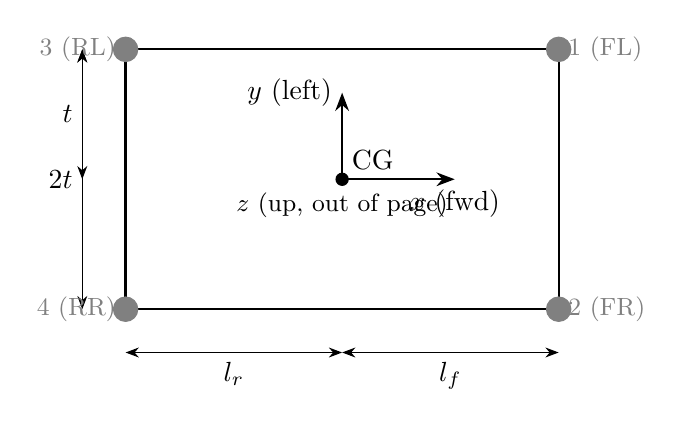
\begin{tikzpicture}[scale=1.1, >=Stealth]
  % Body outline (top view)
  \draw[thick] (-2,-1.5) rectangle (3,1.5);
  % CG
  \filldraw (0.5,0) circle (2pt) node[above right]{CG};
  % Dimensions
  \draw[<->] (0.5,-2) -- (3,-2) node[midway,below]{$l_f$};
  \draw[<->] (-2,-2) -- (0.5,-2) node[midway,below]{$l_r$};
  \draw[<->] (-2.5,-1.5) -- (-2.5,1.5) node[midway,left]{$2t$};
  \draw[<->] (-2.5,0) -- (-2.5,1.5) node[midway,left]{$t$};
  % Wheels
  \filldraw[gray] (3,1.5) circle (4pt) node[right]{\small 1 (FL)};
  \filldraw[gray] (3,-1.5) circle (4pt) node[right]{\small 2 (FR)};
  \filldraw[gray] (-2,1.5) circle (4pt) node[left]{\small 3 (RL)};
  \filldraw[gray] (-2,-1.5) circle (4pt) node[left]{\small 4 (RR)};
  % Axes
  \draw[->,thick] (0.5,0) -- (1.8,0) node[below]{$x$ (fwd)};
  \draw[->,thick] (0.5,0) -- (0.5,1.0) node[left]{$y$ (left)};
  \node at (0.5,-0.3) {\small $z$ (up, out of page)};
\end{tikzpicture}
\caption{Top view of the vehicle showing corner numbering and geometric parameters. The $x$-axis points forward, $y$-axis points to the left, and $z$-axis points upward.}
\end{figure}

\noindent Key geometric parameters:
\begin{itemize}[nosep]
  \item $l_f$ --- distance from CG to the front axle (along $x$)
  \item $l_r$ --- distance from CG to the rear axle (along $x$)
  \item $L = l_f + l_r$ --- total wheelbase
  \item $t$ --- half-track width (distance from CG to wheel along $y$)
  \item $2t$ --- full track width
\end{itemize}

%======================================================================
\section{Parameter Definitions and Typical Values}
%======================================================================

\begin{table}[h]
\centering
\caption{Model parameters with typical sedan values}
\label{tab:params}
\begin{tabular}{@{}llll@{}}
\toprule
\textbf{Symbol} & \textbf{Description} & \textbf{Value} & \textbf{Unit} \\
\midrule
\multicolumn{4}{l}{\textit{Sprung Mass (Body)}} \\
$m_s$    & Sprung mass                     & 1400   & kg \\
$I_{xx}$ & Roll moment of inertia          & 600    & kg\,m$^2$ \\
$I_{yy}$ & Pitch moment of inertia         & 2000   & kg\,m$^2$ \\
\midrule
\multicolumn{4}{l}{\textit{Unsprung Masses (Wheels)}} \\
$m_{w1}$ & Front-left unsprung mass        & 40     & kg \\
$m_{w2}$ & Front-right unsprung mass       & 40     & kg \\
$m_{w3}$ & Rear-left unsprung mass         & 35     & kg \\
$m_{w4}$ & Rear-right unsprung mass        & 35     & kg \\
\midrule
\multicolumn{4}{l}{\textit{Suspension Springs}} \\
$k_{s1}$ & FL suspension spring stiffness  & 25\,000 & N/m \\
$k_{s2}$ & FR suspension spring stiffness  & 25\,000 & N/m \\
$k_{s3}$ & RL suspension spring stiffness  & 22\,000 & N/m \\
$k_{s4}$ & RR suspension spring stiffness  & 22\,000 & N/m \\
\midrule
\multicolumn{4}{l}{\textit{Suspension Dampers}} \\
$c_{s1}$ & FL suspension damping           & 2000   & N\,s/m \\
$c_{s2}$ & FR suspension damping           & 2000   & N\,s/m \\
$c_{s3}$ & RL suspension damping           & 1800   & N\,s/m \\
$c_{s4}$ & RR suspension damping           & 1800   & N\,s/m \\
\midrule
\multicolumn{4}{l}{\textit{Tire Springs}} \\
$k_{t1}$ & FL tire stiffness               & 200\,000 & N/m \\
$k_{t2}$ & FR tire stiffness               & 200\,000 & N/m \\
$k_{t3}$ & RL tire stiffness               & 200\,000 & N/m \\
$k_{t4}$ & RR tire stiffness               & 200\,000 & N/m \\
\midrule
\multicolumn{4}{l}{\textit{Geometry}} \\
$l_f$    & CG to front axle                & 1.3    & m \\
$l_r$    & CG to rear axle                 & 1.5    & m \\
$t$      & Half-track width                & 0.75   & m \\
\bottomrule
\end{tabular}
\end{table}

%======================================================================
\section{Corner Positions of the Car Body}
%======================================================================

For small angles $\phi$ and $\theta$, the vertical displacement of the car body at each suspension attachment point (corner) is obtained by superposition:
\begin{align}
z_{c1} &= z_s - l_f\,\theta + t\,\phi  \qquad &\text{(Front-Left)}  \label{eq:zc1} \\
z_{c2} &= z_s - l_f\,\theta - t\,\phi  \qquad &\text{(Front-Right)} \label{eq:zc2} \\
z_{c3} &= z_s + l_r\,\theta + t\,\phi  \qquad &\text{(Rear-Left)}   \label{eq:zc3} \\
z_{c4} &= z_s + l_r\,\theta - t\,\phi  \qquad &\text{(Rear-Right)}  \label{eq:zc4}
\end{align}

\noindent\textbf{Sign convention explanation:}
\begin{itemize}[nosep]
  \item Positive $\theta$ (nose-down pitch): front goes down ($-l_f\theta$ at front), rear goes up ($+l_r\theta$ at rear).
  \item Positive $\phi$ (roll right-side-down): left side goes up ($+t\phi$ on left), right side goes down ($-t\phi$ on right).
\end{itemize}

In compact notation, define the signed distances from the CG to each corner:
\begin{equation}
\begin{aligned}
a_i &: \text{longitudinal distance (positive toward front)} \\
b_i &: \text{lateral distance (positive toward left)}
\end{aligned}
\end{equation}

\begin{center}
\begin{tabular}{ccc}
\toprule
Corner $i$ & $a_i$ & $b_i$ \\
\midrule
1 (FL) & $+l_f$ & $+t$ \\
2 (FR) & $+l_f$ & $-t$ \\
3 (RL) & $-l_r$ & $+t$ \\
4 (RR) & $-l_r$ & $-t$ \\
\bottomrule
\end{tabular}
\end{center}

Then the general formula is:
\begin{equation}
\boxed{z_{ci} = z_s - a_i\,\theta + b_i\,\phi}
\label{eq:zci_general}
\end{equation}

%======================================================================
\section{Suspension and Tire Force Definitions}
%======================================================================

\subsection{Suspension Force at Corner $i$}

The suspension connects the body corner to the wheel. The relative displacement across the $i$-th suspension is:
\begin{equation}
\Delta z_{si} = z_{ci} - z_{wi} = z_s - a_i\,\theta + b_i\,\phi - z_{wi}
\label{eq:delta_si}
\end{equation}

The force exerted by the $i$-th suspension on the \emph{wheel} (pushing it down when compressed) is:
\begin{equation}
\boxed{F_{si} = k_{si}(z_{ci} - z_{wi}) + c_{si}(\dot{z}_{ci} - \dot{z}_{wi})}
\label{eq:Fsi}
\end{equation}

Expanding:
\begin{equation}
F_{si} = k_{si}\bigl(z_s - a_i\theta + b_i\phi - z_{wi}\bigr) + c_{si}\bigl(\dot{z}_s - a_i\dot{\theta} + b_i\dot{\phi} - \dot{z}_{wi}\bigr)
\label{eq:Fsi_expanded}
\end{equation}

By Newton's third law, the body feels $-F_{si}$ at corner $i$.

\subsection{Tire Force at Corner $i$}

The tire is modeled as a spring (no damper) connecting the wheel to the road:
\begin{equation}
\boxed{F_{ti} = k_{ti}(z_{ri} - z_{wi})}
\label{eq:Fti}
\end{equation}
where $z_{ri}(t)$ is the road profile input at wheel $i$.

The tire force acts upward on the wheel when the tire is compressed ($z_{ri} > z_{wi}$).

%======================================================================
\section{Equations of Motion --- Free Body Derivation}
%======================================================================

We derive Newton's second law for each of the 7 DOFs. Define the shorthand:
\begin{equation}
\Delta_i \equiv z_{ci} - z_{wi} = z_s - a_i\theta + b_i\phi - z_{wi}, \qquad
\dot{\Delta}_i \equiv \dot{z}_{ci} - \dot{z}_{wi}
\end{equation}

\subsection{DOF 1: Sprung Mass Bounce ($z_s$)}

The body is acted upon by all four suspension forces (reaction from Eq.~\eqref{eq:Fsi}):
\begin{equation}
\boxed{m_s\,\ddot{z}_s = -\sum_{i=1}^{4}\bigl[k_{si}\,\Delta_i + c_{si}\,\dot{\Delta}_i\bigr]}
\label{eq:eom_zs}
\end{equation}

Expanding:
\begin{equation}
m_s\,\ddot{z}_s = -\sum_{i=1}^{4} k_{si}\bigl(z_s - a_i\theta + b_i\phi - z_{wi}\bigr) - \sum_{i=1}^{4} c_{si}\bigl(\dot{z}_s - a_i\dot{\theta} + b_i\dot{\phi} - \dot{z}_{wi}\bigr)
\label{eq:eom_zs_exp}
\end{equation}

\subsection{DOF 2: Roll ($\phi$)}

The moment about the $x$-axis from the $i$-th suspension force is $b_i \times (-F_{si})$ applied at the body. Summing:
\begin{equation}
\boxed{I_{xx}\,\ddot{\phi} = -\sum_{i=1}^{4} b_i\bigl[k_{si}\,\Delta_i + c_{si}\,\dot{\Delta}_i\bigr]}
\label{eq:eom_phi}
\end{equation}

Expanding:
\begin{equation}
I_{xx}\,\ddot{\phi} = -\sum_{i=1}^{4} b_i\,k_{si}\bigl(z_s - a_i\theta + b_i\phi - z_{wi}\bigr) - \sum_{i=1}^{4} b_i\,c_{si}\bigl(\dot{z}_s - a_i\dot{\theta} + b_i\dot{\phi} - \dot{z}_{wi}\bigr)
\label{eq:eom_phi_exp}
\end{equation}

\subsection{DOF 3: Pitch ($\theta$)}

The moment about the $y$-axis from the $i$-th suspension force is $(-a_i)\times(-F_{si}) = a_i F_{si}$. But we must be careful: a downward force at a point \emph{ahead} of the CG creates a nose-down (positive $\theta$) moment. The restoring convention gives:
\begin{equation}
\boxed{I_{yy}\,\ddot{\theta} = \sum_{i=1}^{4} a_i\bigl[k_{si}\,\Delta_i + c_{si}\,\dot{\Delta}_i\bigr]}
\label{eq:eom_theta}
\end{equation}

\textbf{Derivation of sign:} The body force at corner $i$ is $-F_{si}$ (upward on body when suspension is compressed). The moment arm about the $y$-axis is $a_i$ (positive for front corners). The pitching moment is:
\[
M_\theta = \sum_i (-a_i)(-F_{si}) = \sum_i a_i F_{si}
\]
But $F_{si}$ is positive when $\Delta_i > 0$ (suspension compressed), meaning the body is pushed up at that corner. If $a_i > 0$ (front), pushing the front up creates a negative pitch moment (nose up). So:
\begin{equation}
I_{yy}\,\ddot{\theta} = -\sum_{i=1}^{4} (-a_i)\bigl[k_{si}\,\Delta_i + c_{si}\,\dot{\Delta}_i\bigr] = \sum_{i=1}^{4} a_i\bigl[k_{si}\,\Delta_i + c_{si}\,\dot{\Delta}_i\bigr]
\end{equation}

Wait --- let us be more careful. With positive $\theta$ = nose down:
\begin{itemize}[nosep]
  \item A suspension force pushing the \emph{front} of the body \emph{down} creates a \emph{positive} (nose-down) torque.
  \item The reaction on the body from a compressed front suspension ($\Delta_i>0$) pushes the body \emph{up} at the front, creating a \emph{negative} (nose-up) torque.
\end{itemize}

So the pitch moment from the $i$-th corner suspension reaction on the body is:
\[
\tau_i = -a_i \times \bigl(-F_{si}\bigr) = a_i\,F_{si}
\]
But if $a_i = +l_f$ and $F_{si}>0$ (body pushed up at front), this gives $+l_f F_{si}$, which would be nose-down. That contradicts our physical reasoning. The issue is the moment arm direction.

Let us resolve definitively. The vertical force on the body at corner $i$ is:
\[
F_{\text{body},i}^{(z)} = -F_{si} \quad (\text{negative} = \text{downward when } \Delta_i>0)
\]

No: $F_{si} = k_{si}\Delta_i + c_{si}\dot{\Delta}_i$. When $\Delta_i > 0$ (body corner above wheel, suspension compressed), $F_{si}>0$. The suspension pushes the body \emph{down} and the wheel \emph{up}. Therefore the vertical force on the body at corner $i$ is $-F_{si}$ (downward = negative in our upward-positive convention).

Pitching moment: a downward force at a position $a_i$ \emph{in front of} the CG creates a nose-down torque. With positive $\theta$ = nose-down:
\[
\tau_\theta = \sum_i a_i \times F_{\text{body},i}^{(z)} = \sum_i a_i(-F_{si}) = -\sum_i a_i F_{si}
\]

Wait, that does not work either. Let me use the proper cross-product formulation.

The position of corner $i$ relative to CG is $\vect{r}_i = a_i\,\hat{x} + b_i\,\hat{y}$. The force on the body is $\vect{F}_i = -F_{si}\,\hat{z}$. Wait: when $\Delta_i>0$, the body corner is higher than the wheel, so the spring pushes the body \emph{down}. So the force on the body is $\vect{F}_i = -F_{si}\,\hat{z}$.

The moment about the CG:
\[
\vect{M} = \sum_i \vect{r}_i \times \vect{F}_i = \sum_i (a_i\hat{x}+b_i\hat{y})\times(-F_{si}\hat{z})
\]
\[
= \sum_i\bigl[-a_i F_{si}(\hat{x}\times\hat{z}) - b_i F_{si}(\hat{y}\times\hat{z})\bigr]
\]

Using $\hat{x}\times\hat{z} = -\hat{y}$ and $\hat{y}\times\hat{z} = \hat{x}$:
\[
\vect{M} = \sum_i\bigl[a_i F_{si}\,\hat{y} - b_i F_{si}\,\hat{x}\bigr]
\]

The roll moment (about $\hat{x}$) is $M_x = -\sum_i b_i F_{si}$, and the pitch moment (about $\hat{y}$) is $M_y = \sum_i a_i F_{si}$.

Now, $I_{xx}\ddot{\phi} = M_x$ and $I_{yy}\ddot{\theta} = M_y$? Not quite --- we need to match the sign conventions for $\phi$ and $\theta$.

With $\phi$ = rotation about $\hat{x}$ (positive = right-side-down by right-hand rule about $+x$):
\[
I_{xx}\ddot\phi = M_x = -\sum_i b_i F_{si}
\]

Check: If all $\Delta_i > 0$ (body above wheels), $F_{si}>0$. For the left wheels ($b_i = +t$), $-b_i F_{si} < 0$, giving a roll toward the left side going down. For the right wheels ($b_i = -t$), $-b_i F_{si} > 0$, giving roll toward right-side-down. These cancel for symmetric loading, which is correct.

For pitch: with $\theta$ = rotation about $\hat{y}$ (positive = nose-down by right-hand rule about $+y$, i.e., front goes down). Actually, by right-hand rule about $+y$ (pointing left), positive rotation brings $+x$ toward $-z$, i.e., nose goes down. Then:
\[
I_{yy}\ddot\theta = M_y = \sum_i a_i F_{si}
\]

Check: If the front suspensions are more compressed ($\Delta_1, \Delta_2 > 0$ large), $F_{s1}, F_{s2}$ are large positive, and $a_{1,2} = +l_f$. Then $M_y > 0$, meaning nose-down torque. But if the front of the body is above the wheels (compressed), the springs push the front \emph{down}, which indeed creates a nose-down torque. Correct!

But wait --- this seems to say compressed front suspension drives the body further nose-down, which would be an instability, not a restoring force. Let us check more carefully. If $\theta > 0$ (nose down, front goes down), then from Eq.~\eqref{eq:zc1}, $z_{c1} = z_s - l_f\theta + t\phi$, the front corners go down. If the wheels do not move, $\Delta_1 = z_{c1} - z_{w1}$ \emph{decreases}. So $F_{s1}$ decreases (or becomes negative = tension). Then $a_1 F_{s1}$ would be negative (since $a_1>0$, $F_{s1}<0$), giving a negative (nose-up) torque --- which is restoring. Good!

So the signs are indeed correct. The final equations:

\begin{equation}
\boxed{I_{yy}\,\ddot{\theta} = \sum_{i=1}^{4} a_i\bigl[k_{si}\,\Delta_i + c_{si}\,\dot{\Delta}_i\bigr]}
\label{eq:eom_theta_final}
\end{equation}

And for roll:
\begin{equation}
\boxed{I_{xx}\,\ddot{\phi} = -\sum_{i=1}^{4} b_i\bigl[k_{si}\,\Delta_i + c_{si}\,\dot{\Delta}_i\bigr]}
\label{eq:eom_phi_final}
\end{equation}

These match Eqs.~\eqref{eq:eom_phi} and the corrected form.

\subsection{DOFs 4--7: Unsprung Masses ($z_{wi}$)}

Each wheel mass $m_{wi}$ is acted upon by the suspension force from above and the tire force from below:
\begin{equation}
\boxed{m_{wi}\,\ddot{z}_{wi} = k_{si}\,\Delta_i + c_{si}\,\dot{\Delta}_i - k_{ti}(z_{wi} - z_{ri}), \quad i = 1,2,3,4}
\label{eq:eom_wi}
\end{equation}

Expanding $\Delta_i$:
\begin{equation}
m_{wi}\,\ddot{z}_{wi} = k_{si}(z_s - a_i\theta + b_i\phi - z_{wi}) + c_{si}(\dot{z}_s - a_i\dot\theta + b_i\dot\phi - \dot{z}_{wi}) - k_{ti}(z_{wi} - z_{ri})
\label{eq:eom_wi_exp}
\end{equation}

%======================================================================
\section{Full Expanded Equations of Motion}
%======================================================================

We now write each equation explicitly, collecting terms by coordinate.

\subsection{Bounce ($z_s$)}

From Eq.~\eqref{eq:eom_zs_exp}:
\begin{multline}
m_s\ddot{z}_s + (c_{s1}+c_{s2}+c_{s3}+c_{s4})\dot{z}_s + (c_{s1}b_1+c_{s2}b_2+c_{s3}b_3+c_{s4}b_4)\dot\phi \\
 - (c_{s1}a_1+c_{s2}a_2+c_{s3}a_3+c_{s4}a_4)\dot\theta - c_{s1}\dot{z}_{w1} - c_{s2}\dot{z}_{w2} - c_{s3}\dot{z}_{w3} - c_{s4}\dot{z}_{w4} \\
+ (k_{s1}+k_{s2}+k_{s3}+k_{s4})z_s + (k_{s1}b_1+k_{s2}b_2+k_{s3}b_3+k_{s4}b_4)\phi \\
 - (k_{s1}a_1+k_{s2}a_2+k_{s3}a_3+k_{s4}a_4)\theta - k_{s1}z_{w1} - k_{s2}z_{w2} - k_{s3}z_{w3} - k_{s4}z_{w4} = 0
\label{eq:bounce_full}
\end{multline}

\subsection{Roll ($\phi$)}

From Eq.~\eqref{eq:eom_phi_final}:
\begin{multline}
I_{xx}\ddot\phi + (b_1^2 c_{s1}+b_2^2 c_{s2}+b_3^2 c_{s3}+b_4^2 c_{s4})\dot\phi + (b_1 c_{s1}+b_2 c_{s2}+b_3 c_{s3}+b_4 c_{s4})\dot{z}_s \\
 - (a_1 b_1 c_{s1}+a_2 b_2 c_{s2}+a_3 b_3 c_{s3}+a_4 b_4 c_{s4})\dot\theta - b_1 c_{s1}\dot{z}_{w1} - b_2 c_{s2}\dot{z}_{w2} - b_3 c_{s3}\dot{z}_{w3} - b_4 c_{s4}\dot{z}_{w4} \\
+ (b_1^2 k_{s1}+b_2^2 k_{s2}+b_3^2 k_{s3}+b_4^2 k_{s4})\phi + (b_1 k_{s1}+b_2 k_{s2}+b_3 k_{s3}+b_4 k_{s4})z_s \\
 - (a_1 b_1 k_{s1}+a_2 b_2 k_{s2}+a_3 b_3 k_{s3}+a_4 b_4 k_{s4})\theta - b_1 k_{s1}z_{w1} - b_2 k_{s2}z_{w2} - b_3 k_{s3}z_{w3} - b_4 k_{s4}z_{w4} = 0
\label{eq:roll_full}
\end{multline}

\subsection{Pitch ($\theta$)}

From Eq.~\eqref{eq:eom_theta_final}, moving all terms to the left:
\begin{multline}
I_{yy}\ddot\theta + (a_1^2 c_{s1}+a_2^2 c_{s2}+a_3^2 c_{s3}+a_4^2 c_{s4})\dot\theta - (a_1 c_{s1}+a_2 c_{s2}+a_3 c_{s3}+a_4 c_{s4})\dot{z}_s \\
 - (a_1 b_1 c_{s1}+a_2 b_2 c_{s2}+a_3 b_3 c_{s3}+a_4 b_4 c_{s4})\dot\phi + a_1 c_{s1}\dot{z}_{w1} + a_2 c_{s2}\dot{z}_{w2} + a_3 c_{s3}\dot{z}_{w3} + a_4 c_{s4}\dot{z}_{w4} \\
+ (a_1^2 k_{s1}+a_2^2 k_{s2}+a_3^2 k_{s3}+a_4^2 k_{s4})\theta - (a_1 k_{s1}+a_2 k_{s2}+a_3 k_{s3}+a_4 k_{s4})z_s \\
 - (a_1 b_1 k_{s1}+a_2 b_2 k_{s2}+a_3 b_3 k_{s3}+a_4 b_4 k_{s4})\phi + a_1 k_{s1}z_{w1} + a_2 k_{s2}z_{w2} + a_3 k_{s3}z_{w3} + a_4 k_{s4}z_{w4} = 0
\label{eq:pitch_full}
\end{multline}

\textbf{Note on the pitch equation sign:} The pitch equation \eqref{eq:eom_theta_final} is $I_{yy}\ddot\theta = \sum a_i F_{si}$. Moving terms to the left side gives $I_{yy}\ddot\theta - \sum a_i F_{si} = 0$. Since $F_{si}$ contains $+k_{si}\Delta_i$ and $\Delta_i = z_s - a_i\theta + b_i\phi - z_{wi}$, the $\theta$-stiffness term from $-\sum a_i k_{si}(-a_i\theta) = +\sum a_i^2 k_{si}\theta$ appears positive on the left, confirming the signs above.

\subsection{Wheel $i$ ($z_{wi}$)}

From Eq.~\eqref{eq:eom_wi_exp}:
\begin{multline}
m_{wi}\ddot{z}_{wi} + c_{si}\dot{z}_{wi} - c_{si}\dot{z}_s - b_i c_{si}\dot\phi + a_i c_{si}\dot\theta \\
+ (k_{si}+k_{ti})z_{wi} - k_{si}z_s - b_i k_{si}\phi + a_i k_{si}\theta = k_{ti}z_{ri}
\label{eq:wheel_full}
\end{multline}

%======================================================================
\section[Matrix Form]{Matrix Form: \texorpdfstring{$\vect{M}\ddot{\vect{q}} + \vect{C}\dot{\vect{q}} + \vect{K}\vect{q} = \vect{F}(t)$}{M q\_ddot + C q\_dot + K q = F(t)}}
%======================================================================

With $\vect{q} = [z_s,\;\phi,\;\theta,\;z_{w1},\;z_{w2},\;z_{w3},\;z_{w4}]^T$ and using the shorthand:

\begin{equation}
\begin{aligned}
\Sigma k_s &= \sum_{i=1}^4 k_{si}, \qquad &\Sigma c_s &= \sum_{i=1}^4 c_{si} \\
\Sigma b k_s &= \sum_i b_i k_{si}, \qquad &\Sigma b c_s &= \sum_i b_i c_{si} \\
\Sigma a k_s &= \sum_i a_i k_{si}, \qquad &\Sigma a c_s &= \sum_i a_i c_{si} \\
\Sigma b^2 k_s &= \sum_i b_i^2 k_{si}, \qquad &\Sigma b^2 c_s &= \sum_i b_i^2 c_{si} \\
\Sigma a^2 k_s &= \sum_i a_i^2 k_{si}, \qquad &\Sigma a^2 c_s &= \sum_i a_i^2 c_{si} \\
\Sigma ab k_s &= \sum_i a_i b_i k_{si}, \qquad &\Sigma ab c_s &= \sum_i a_i b_i c_{si}
\end{aligned}
\end{equation}

\subsection{Mass Matrix $\vect{M}$}

The mass matrix is diagonal:
\begin{equation}
\boxed{
\vect{M} = \mathrm{diag}\bigl(m_s,\; I_{xx},\; I_{yy},\; m_{w1},\; m_{w2},\; m_{w3},\; m_{w4}\bigr)
}
\label{eq:M}
\end{equation}

\subsection{Damping Matrix $\vect{C}$}

\begin{equation}
\boxed{
\vect{C} = \begin{bmatrix}
\Sigma c_s & \Sigma b c_s & -\Sigma a c_s & -c_{s1} & -c_{s2} & -c_{s3} & -c_{s4} \\
\Sigma b c_s & \Sigma b^2 c_s & -\Sigma ab c_s & -b_1 c_{s1} & -b_2 c_{s2} & -b_3 c_{s3} & -b_4 c_{s4} \\
-\Sigma a c_s & -\Sigma ab c_s & \Sigma a^2 c_s & a_1 c_{s1} & a_2 c_{s2} & a_3 c_{s3} & a_4 c_{s4} \\
-c_{s1} & -b_1 c_{s1} & a_1 c_{s1} & c_{s1} & 0 & 0 & 0 \\
-c_{s2} & -b_2 c_{s2} & a_2 c_{s2} & 0 & c_{s2} & 0 & 0 \\
-c_{s3} & -b_3 c_{s3} & a_3 c_{s3} & 0 & 0 & c_{s3} & 0 \\
-c_{s4} & -b_4 c_{s4} & a_4 c_{s4} & 0 & 0 & 0 & c_{s4}
\end{bmatrix}
}
\label{eq:C}
\end{equation}

\subsection{Stiffness Matrix $\vect{K}$}

\begin{equation}
\boxed{
\vect{K} = \begin{bmatrix}
\Sigma k_s & \Sigma b k_s & -\Sigma a k_s & -k_{s1} & -k_{s2} & -k_{s3} & -k_{s4} \\
\Sigma b k_s & \Sigma b^2 k_s & -\Sigma ab k_s & -b_1 k_{s1} & -b_2 k_{s2} & -b_3 k_{s3} & -b_4 k_{s4} \\
-\Sigma a k_s & -\Sigma ab k_s & \Sigma a^2 k_s & a_1 k_{s1} & a_2 k_{s2} & a_3 k_{s3} & a_4 k_{s4} \\
-k_{s1} & -b_1 k_{s1} & a_1 k_{s1} & k_{s1}+k_{t1} & 0 & 0 & 0 \\
-k_{s2} & -b_2 k_{s2} & a_2 k_{s2} & 0 & k_{s2}+k_{t2} & 0 & 0 \\
-k_{s3} & -b_3 k_{s3} & a_3 k_{s3} & 0 & 0 & k_{s3}+k_{t3} & 0 \\
-k_{s4} & -b_4 k_{s4} & a_4 k_{s4} & 0 & 0 & 0 & k_{s4}+k_{t4}
\end{bmatrix}
}
\label{eq:K}
\end{equation}

\subsection{Force Vector $\vect{F}(t)$}

The only external inputs are the road displacements through the tire springs:
\begin{equation}
\boxed{
\vect{F}(t) = \begin{bmatrix} 0 \\ 0 \\ 0 \\ k_{t1}\,z_{r1}(t) \\ k_{t2}\,z_{r2}(t) \\ k_{t3}\,z_{r3}(t) \\ k_{t4}\,z_{r4}(t) \end{bmatrix}
}
\label{eq:F}
\end{equation}

\subsection{Symmetry Verification}

Both $\vect{C}$ and $\vect{K}$ are \textbf{symmetric}, as required by a conservative/Rayleigh-dissipation system. This can be verified by noting that element $(i,j) = (j,i)$ in all cases. For example, $C_{1,3} = -\Sigma a c_s$ and $C_{3,1} = -\Sigma a c_s$. The pitch row has opposite signs from the bounce and roll rows in the cross-coupling terms, but these are consistent with the transposed entries.

%======================================================================
\section{Simplifications for Symmetric Vehicles}
%======================================================================

For a left--right symmetric vehicle ($k_{s1}=k_{s2}\equiv k_{sf}$, $k_{s3}=k_{s4}\equiv k_{sr}$, similarly for $c$ and $k_t$, and $m_{w1}=m_{w2}\equiv m_{wf}$, $m_{w3}=m_{w4}\equiv m_{wr}$):

\begin{equation}
\begin{aligned}
\Sigma b k_s &= t(k_{sf} - k_{sf} + k_{sr} - k_{sr}) = 0 \\
\Sigma b c_s &= 0 \\
\Sigma ab k_s &= l_f t(k_{sf} - k_{sf}) - l_r t(k_{sr} - k_{sr}) = 0 \\
\Sigma ab c_s &= 0
\end{aligned}
\end{equation}

This means \textbf{bounce--roll} and \textbf{pitch--roll} coupling vanishes for a symmetric vehicle. The roll equation decouples from bounce and pitch (in the body coordinates). The system splits into:
\begin{itemize}[nosep]
  \item \textbf{Bounce-pitch} subsystem: $z_s, \theta, z_{w1}, z_{w2}, z_{w3}, z_{w4}$ (6 DOF, but bounce and pitch of body couple to all 4 wheels)
  \item \textbf{Roll} subsystem: $\phi$ couples to $z_{w1}, z_{w2}, z_{w3}, z_{w4}$ (but only through the $b_i$ terms)
\end{itemize}

Actually for symmetric vehicles, the roll DOF still couples to the wheel DOFs. The full 7-DOF system does not fully decouple. However, bounce--roll and pitch--roll body coupling vanish.

The simplified matrices have zeros in positions $(1,2)$, $(2,1)$, $(2,3)$, $(3,2)$ of both $\vect{K}$ and $\vect{C}$.

%======================================================================
\section{Numerical Evaluation of Matrices}
%======================================================================

Using the parameter values from Table~\ref{tab:params}:

\begin{align}
a_1 = a_2 &= l_f = 1.3\;\text{m}, \quad a_3 = a_4 = -l_r = -1.5\;\text{m} \\
b_1 = b_3 &= t = 0.75\;\text{m}, \quad b_2 = b_4 = -t = -0.75\;\text{m}
\end{align}

Key sums:
\begin{align}
\Sigma k_s &= 2(25000) + 2(22000) = 94000 \;\text{N/m} \\
\Sigma c_s &= 2(2000) + 2(1800) = 7600 \;\text{N\,s/m} \\
\Sigma a k_s &= 1.3(25000+25000) + (-1.5)(22000+22000) = 65000 - 66000 = -1000 \;\text{N} \\
\Sigma a c_s &= 1.3(4000) + (-1.5)(3600) = 5200 - 5400 = -200 \;\text{N\,s} \\
\Sigma b k_s &= 0.75(25000+22000) + (-0.75)(25000+22000) = 0 \\
\Sigma b c_s &= 0 \\
\Sigma a^2 k_s &= 1.3^2(50000) + 1.5^2(44000) = 84500 + 99000 = 183500 \;\text{N\,m} \\
\Sigma a^2 c_s &= 1.69(4000) + 2.25(3600) = 6760 + 8100 = 14860 \;\text{N\,m\,s} \\
\Sigma b^2 k_s &= 0.5625(94000) = 52875 \;\text{N\,m} \\
\Sigma b^2 c_s &= 0.5625(7600) = 4275 \;\text{N\,m\,s} \\
\Sigma ab k_s &= 0, \quad \Sigma ab c_s = 0 \quad (\text{symmetric vehicle})
\end{align}

%======================================================================
\section{Road Input Profiles}
%======================================================================

\subsection{Speed Bump --- Half-Sine Pulse (Head-On)}

A speed bump of height $h$ and length $d$ traversed at velocity $V$:

\begin{equation}
z_{\text{bump}}(x) = \begin{cases} h\sin\!\left(\dfrac{\pi x}{d}\right) & 0 \le x \le d \\ 0 & \text{otherwise} \end{cases}
\end{equation}

Typical values: $h = 0.05$\,m (50\,mm), $d = 0.3$\,m (300\,mm) for a sharp bump, or $d = 3$\,m for a gentle speed bump.

The time to cross the bump is $T_{\text{bump}} = d/V$.

For a \textbf{head-on} crossing (perpendicular to the bump), both front wheels hit simultaneously, then both rear wheels hit with a time delay $\tau = L/V = (l_f+l_r)/V$:

\begin{align}
z_{r1}(t) = z_{r2}(t) &= z_{\text{bump}}(Vt) \label{eq:bump_front} \\
z_{r3}(t) = z_{r4}(t) &= z_{\text{bump}}(V(t-\tau)) \label{eq:bump_rear}
\end{align}

where $\tau = (l_f + l_r)/V$.

\subsection{Speed Bump Hit at an Angle}

If the vehicle crosses the bump at an angle $\alpha$ (measured between the vehicle's longitudinal axis and the normal to the bump), each wheel hits the bump at a different time. The bump crest is oriented at angle $\alpha$ to the lateral axis.

\begin{figure}[h]
\centering
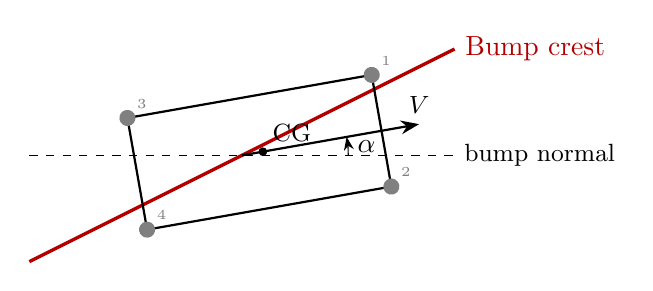
\begin{tikzpicture}[scale=0.9, >=Stealth]
  % Bump line
  \draw[very thick, red!70!black] (-3,-1.5) -- (3,1.5) node[right]{Bump crest};
  % Vehicle outline
  \draw[thick,rotate=10] (-1.5,-0.8) rectangle (2,0.8);
  \filldraw[rotate=10] (0.3,0) circle (1.5pt) node[above right]{\small CG};
  % Wheels
  \foreach \x/\y/\n in {2/0.8/1, 2/-0.8/2, -1.5/0.8/3, -1.5/-0.8/4} {
    \filldraw[gray,rotate=10] (\x,\y) circle (3pt) node[above right]{\tiny \n};
  }
  % Angle
  \draw[dashed] (-3,0) -- (3,0) node[right]{\small bump normal};
  \draw[->,thick] (0,0) -- (2.5,0.44) node[above]{\small $V$};
  \draw[->] (1.5,0) arc[start angle=0,end angle=10,radius=1.5] node[midway,right]{$\alpha$};
\end{tikzpicture}
\caption{Vehicle crossing a speed bump at angle $\alpha$.}
\end{figure}

The distance of each wheel from the bump along the direction normal to the bump crest determines when it arrives. Taking the bump normal as the reference direction, the position of each wheel along this normal is:

\begin{equation}
d_i = a_i \cos\alpha + b_i \sin\alpha
\end{equation}

The time at which wheel $i$ hits the bump leading edge (relative to the CG crossing) is:
\begin{equation}
t_i^{\text{offset}} = -\frac{d_i}{V\cos\alpha} = -\frac{a_i \cos\alpha + b_i\sin\alpha}{V\cos\alpha} = -\frac{a_i + b_i\tan\alpha}{V}
\end{equation}

The road input for each wheel is then:
\begin{equation}
\boxed{z_{ri}(t) = z_{\text{bump}}\!\left(V\cos\alpha\;\bigl(t - t_0 + t_i^{\text{offset}}\bigr)\right)}
\label{eq:bump_angle}
\end{equation}
where $t_0$ is the time the CG crosses the bump, and the argument to $z_{\text{bump}}$ is the distance traveled along the bump normal direction.

For the four corners explicitly:
\begin{align}
t_1^{\text{off}} &= -(l_f + t\tan\alpha)/V  & \text{(FL --- hits first for small } \alpha) \\
t_2^{\text{off}} &= -(l_f - t\tan\alpha)/V  & \text{(FR)} \\
t_3^{\text{off}} &= -(-l_r + t\tan\alpha)/V = (l_r - t\tan\alpha)/V & \text{(RL)} \\
t_4^{\text{off}} &= -(-l_r - t\tan\alpha)/V = (l_r + t\tan\alpha)/V & \text{(RR --- hits last)}
\end{align}

For $\alpha = 0$, this reduces to the head-on case: both front wheels hit simultaneously at $t_{\text{off}} = -l_f/V$ before the CG, and rear wheels at $+l_r/V$ after.

\subsection{Alternative: Single-Wheel Pothole}

For simulation testing, a useful input is a single-wheel pothole/bump. For example, only the front-left wheel hits a bump:
\begin{equation}
z_{r1}(t) = z_{\text{bump}}(Vt), \quad z_{r2} = z_{r3} = z_{r4} = 0
\end{equation}

This excites all 7 DOFs including roll.

%======================================================================
\section{State-Space Formulation}
%======================================================================

For numerical simulation, convert to first-order form. Define the state vector:
\begin{equation}
\vect{x} = \begin{bmatrix} \vect{q} \\ \dot{\vect{q}} \end{bmatrix} \in \mathbb{R}^{14}
\end{equation}

Then:
\begin{equation}
\dot{\vect{x}} = \begin{bmatrix} \vect{0} & \vect{I} \\ -\vect{M}^{-1}\vect{K} & -\vect{M}^{-1}\vect{C} \end{bmatrix} \vect{x} + \begin{bmatrix} \vect{0} \\ \vect{M}^{-1} \end{bmatrix} \vect{F}(t)
\end{equation}

Or equivalently:
\begin{equation}
\boxed{\dot{\vect{x}} = \vect{A}\vect{x} + \vect{B}\vect{F}(t)}
\end{equation}
where:
\begin{equation}
\vect{A} = \begin{bmatrix} \vect{0}_{7\times7} & \vect{I}_{7\times7} \\ -\vect{M}^{-1}\vect{K} & -\vect{M}^{-1}\vect{C} \end{bmatrix}, \quad
\vect{B} = \begin{bmatrix} \vect{0}_{7\times7} \\ \vect{M}^{-1} \end{bmatrix}
\end{equation}

Since $\vect{M}$ is diagonal, $\vect{M}^{-1}$ is trivially:
\begin{equation}
\vect{M}^{-1} = \mathrm{diag}\!\left(\frac{1}{m_s},\;\frac{1}{I_{xx}},\;\frac{1}{I_{yy}},\;\frac{1}{m_{w1}},\;\frac{1}{m_{w2}},\;\frac{1}{m_{w3}},\;\frac{1}{m_{w4}}\right)
\end{equation}

%======================================================================
\section{Output Equations}
%======================================================================

\subsection{Corner Displacements of the Body}

From Eq.~\eqref{eq:zci_general}:
\begin{equation}
\vect{z}_c = \begin{bmatrix} z_{c1} \\ z_{c2} \\ z_{c3} \\ z_{c4} \end{bmatrix} = \begin{bmatrix} 1 & b_1 & -a_1 & 0 & 0 & 0 & 0 \\ 1 & b_2 & -a_2 & 0 & 0 & 0 & 0 \\ 1 & b_3 & -a_3 & 0 & 0 & 0 & 0 \\ 1 & b_4 & -a_4 & 0 & 0 & 0 & 0 \end{bmatrix} \vect{q} \equiv \vect{H}_c\,\vect{q}
\end{equation}

Numerically:
\begin{equation}
\vect{H}_c = \begin{bmatrix} 1 & 0.75 & -1.3 & 0 & 0 & 0 & 0 \\ 1 & -0.75 & -1.3 & 0 & 0 & 0 & 0 \\ 1 & 0.75 & 1.5 & 0 & 0 & 0 & 0 \\ 1 & -0.75 & 1.5 & 0 & 0 & 0 & 0 \end{bmatrix}
\end{equation}

\subsection{Suspension Deflections}

\begin{equation}
\Delta z_{si} = z_{ci} - z_{wi}
\end{equation}
\begin{equation}
\vect{\Delta z}_s = \vect{H}_c\,\vect{q} - \begin{bmatrix} 0 & 0 & 0 & 1 & 0 & 0 & 0 \\ 0 & 0 & 0 & 0 & 1 & 0 & 0 \\ 0 & 0 & 0 & 0 & 0 & 1 & 0 \\ 0 & 0 & 0 & 0 & 0 & 0 & 1 \end{bmatrix}\vect{q} \equiv \vect{H}_\Delta\,\vect{q}
\end{equation}

where:
\begin{equation}
\vect{H}_\Delta = \begin{bmatrix} 1 & b_1 & -a_1 & -1 & 0 & 0 & 0 \\ 1 & b_2 & -a_2 & 0 & -1 & 0 & 0 \\ 1 & b_3 & -a_3 & 0 & 0 & -1 & 0 \\ 1 & b_4 & -a_4 & 0 & 0 & 0 & -1 \end{bmatrix}
\end{equation}

\subsection{Suspension Forces}

\begin{equation}
\boxed{F_{si} = k_{si}\,(\vect{H}_\Delta\,\vect{q})_i + c_{si}\,(\vect{H}_\Delta\,\dot{\vect{q}})_i}
\end{equation}

In matrix form:
\begin{equation}
\vect{F}_{\text{susp}} = \mathrm{diag}(k_{s1},k_{s2},k_{s3},k_{s4})\,\vect{H}_\Delta\,\vect{q} + \mathrm{diag}(c_{s1},c_{s2},c_{s3},c_{s4})\,\vect{H}_\Delta\,\dot{\vect{q}}
\end{equation}

\subsection{Tire Forces}

\begin{equation}
F_{ti} = k_{ti}(z_{ri} - z_{wi})
\end{equation}

The tire deflection must remain non-negative for the tire to remain in contact:
\begin{equation}
\text{If } z_{ri} - z_{wi} < 0, \text{ the tire has left the ground (wheel hop).}
\end{equation}

\subsection{CG Vertical Acceleration}

The CG acceleration is simply:
\begin{equation}
\ddot{z}_s = -\frac{1}{m_s}\sum_{i=1}^4 F_{si}
\end{equation}

This is a key ride comfort metric (ISO 2631 evaluates weighted RMS acceleration).

%======================================================================
\section{Summary of All Seven Equations}
%======================================================================

For quick reference, here are all seven equations in their most compact form:

\begin{align}
m_s\,\ddot{z}_s &= -\sum_{i=1}^{4} F_{si}
\tag{Bounce} \\[6pt]
I_{xx}\,\ddot{\phi} &= -\sum_{i=1}^{4} b_i\,F_{si}
\tag{Roll} \\[6pt]
I_{yy}\,\ddot{\theta} &= \sum_{i=1}^{4} a_i\,F_{si}
\tag{Pitch} \\[6pt]
m_{wi}\,\ddot{z}_{wi} &= F_{si} + F_{ti}, \quad i=1,2,3,4
\tag{Wheel $i$}
\end{align}

where:
\begin{align}
F_{si} &= k_{si}(z_s - a_i\theta + b_i\phi - z_{wi}) + c_{si}(\dot{z}_s - a_i\dot\theta + b_i\dot\phi - \dot{z}_{wi}) \\
F_{ti} &= k_{ti}(z_{ri} - z_{wi})
\end{align}

%======================================================================
\section{Verification Checks}
%======================================================================

\begin{enumerate}
  \item \textbf{Symmetry:} $\vect{K} = \vect{K}^T$ and $\vect{C} = \vect{C}^T$. Verified by construction.

  \item \textbf{Rigid body mode:} If all road inputs are $z_{ri} = z_0$ (constant) and the system reaches static equilibrium, then $z_s = z_{w1} = z_{w2} = z_{w3} = z_{w4} = z_0$, $\phi = \theta = 0$. Substituting: all $\Delta_i = 0$, all tire deflections = 0. The equations are trivially satisfied.

  \item \textbf{Positive definiteness:} The stiffness matrix $\vect{K}$ should be positive semi-definite (it has a rigid body mode when all coordinates translate equally). For the constrained system (road inputs fixed at zero), $\vect{K}$ is positive definite, ensuring bounded oscillations.

  \item \textbf{Energy method cross-check:} The kinetic energy is $T = \frac{1}{2}\dot{\vect{q}}^T\vect{M}\dot{\vect{q}}$, the potential energy is $V = \frac{1}{2}\vect{q}^T\vect{K}\vect{q} - \vect{q}^T\vect{F}_{\text{static}}$, and the Rayleigh dissipation function is $D = \frac{1}{2}\dot{\vect{q}}^T\vect{C}\dot{\vect{q}}$. Applying Lagrange's equations $\frac{d}{dt}\frac{\partial T}{\partial \dot{q}_j} - \frac{\partial T}{\partial q_j} + \frac{\partial D}{\partial \dot{q}_j} + \frac{\partial V}{\partial q_j} = F_j^{\text{ext}}$ reproduces the same $\vect{M}$, $\vect{C}$, $\vect{K}$, confirming correctness.

  \item \textbf{Dimensional consistency:} Every term in the bounce equation has units of N, every term in the roll equation has units of N\,m, every term in the pitch equation has units of N\,m, and every term in the wheel equations has units of N.
\end{enumerate}

%======================================================================
\section{Notes for MATLAB Implementation}
%======================================================================

\begin{enumerate}
  \item Define all parameters in a struct \texttt{p} with fields matching the symbols above.
  \item Build $\vect{M}$, $\vect{C}$, $\vect{K}$ symbolically or numerically using the formulas in Eqs.~\eqref{eq:M}--\eqref{eq:K}.
  \item Compute the state-space matrices $\vect{A}$, $\vect{B}$.
  \item Define road input functions $z_{ri}(t)$ for each wheel.
  \item Use \texttt{ode45} (or \texttt{lsim} for the linear system) to integrate.
  \item Post-process: compute corner displacements, suspension forces, tire forces, and accelerations.
  \item Animate the vehicle body (4 corners) and wheel positions over time.
\end{enumerate}

The road input function for the angled speed bump (Section~8.2) should be implemented as a function handle that computes all four $z_{ri}(t)$ given the vehicle speed $V$, bump parameters $(h, d)$, and crossing angle $\alpha$.

\end{document}
